\documentclass[10pt, titlepage, oneside, a4paper]{article}
%\documentclass{book}


\usepackage[T1]{fontenc}
\usepackage[english]{babel}
\usepackage{amssymb, graphicx}
\usepackage{fancyhdr}
\usepackage{listings}
\usepackage{epstopdf}
\usepackage{hyperref}

\usepackage{times}  
\usepackage{amsmath}
\usepackage{amssymb}
\usepackage{graphicx}
\usepackage{theorem}
\usepackage[latin1]{inputenc}
\usepackage{latexsym}
\usepackage{url}
\usepackage{babel}

\hyphenpenalty=100000


\addtolength{\textheight}{20mm}
\addtolength{\voffset}{-5mm}

\renewcommand{\sectionmark}[1]{\markleft{#1}}
%\renewcommand{\chaptermark}[1]{%

%\markboth{#1}{}} \renewcommand{\sectionmark}[1]{%
%\markright{\thesection\ #1}}

% \Section ger mindre spillutrymme, anv?nd dem om du vill
\newcommand{\Section}[1]{\section{#1}\vspace{-8pt}}
\newcommand{\Subsection}[1]{\vspace{-4pt}\subsection{#1}\vspace{-8pt}}
\newcommand{\Subsubsection}[1]{\vspace{-4pt}\subsubsection{#1}\vspace{-8pt}}
	
% appendices, \appitem och \appsubitem ?r f?r bilagor
\newcounter{appendixpage}

\newenvironment{appendices}{
	\setcounter{appendixpage}{\arabic{page}}
	\stepcounter{appendixpage}
}{
}

\newcommand{\appitem}[2]{
	\stepcounter{section}
	\addtocontents{toc}{\protect\contentsline{section}{\numberline{\Alph{section}}#1}{\arabic{appendixpage}}}
	\addtocounter{appendixpage}{#2}
}

\newcommand{\appsubitem}[2]{
	\stepcounter{subsection}
	\addtocontents{toc}{\protect\contentsline{subsection}{\numberline{\Alph{section}.\arabic{subsection}}#1}{\arabic{appendixpage}}}
	\addtocounter{appendixpage}{#2}
}

\def\inst{Teknik och Naturvetenskap}
\def\course{Fluid Simulation}
\def\pretitle{TNM085 Modelleringsprojekt}
\def\title{TNM085 MODELLERINGSPROJEKT}
\def\graders{Anna Lombardi}


% om du vill referera till katalogen d?r dina filer ligger kan du 
% anv?nda \fullpath som kommer att vara "~username/edu..." o.s.v.
\begin{document}

	% skapar framsidan (om den inte duger: g?r helt enkelt en egen)
	
	\begin{titlepage}

		\thispagestyle{empty}
		
		\begin{large}
			\begin{tabular}{@{}p{\textwidth}@{}}
			
				\textbf{LINK�PINGS UNIVERSITET\hfill} \\
				\textbf{Institutionen f�r \inst} \\
			\end{tabular}
		\end{large}
		\vspace{50mm}
		\begin{center}
			\LARGE{\pretitle} \\
			\huge{\textbf{\course}}\\
			\vspace{10mm}
			
			\vspace{15mm}
			\normalsize\today
			\vspace{15mm}
			
			\begin{large}
			Robert Novo, robno767@student.liu.se\\
			Martin Person, marpe357@student.liu.se\\
			Mattias Persson, matpe621@student.liu.se\\
			Johannes Ullstr�m, johul223@student.liu.se\\
			\end{large}
			
			\vfill
			\large{\textbf{Examiner}}\\
			\mbox{\large{\graders}}
		\end{center}
	\end{titlepage}

	\begin{abstract}
	This report discusses a project which aim was to program an interactive application that uses particle-based visualisation of fluids in real-time. The fluid simulation utilize SPH, which is based on the Navier-Stokes equations. The application is programmed in the program language C\# and uses the environment Microsoft XNA for the visualization.
Keywords: simulation, fluids, Navier-Stokes, SPH, marching cubes, C\#, XNA.
	\end{abstract}

	% fixar sidfot och sidhuvud
%	\lfoot{\footnotesize{\name\course}}
	\lhead{\nouppercase\sc\footnotesize\title}
	\rhead{\nouppercase{\sc\footnotesize}}
	\pagestyle{fancy}
	\renewcommand{\headrulewidth}{0.2pt}
	\renewcommand{\footrulewidth}{0.2pt}

	% skapar inneh�llsf?rteckning.
	% T?nk p� att k?ra latex 2ggr f?r att uppdatera allt
	\tableofcontents
	
	\newpage
	
	\addtocontents{toc}{\protect\thispagestyle{empty}}
	\listoffigures    % chapter with the list of figures
%	\addtocontents{lof}{\protect\thispagestyle{empty}}
%	\listoftables     % chapter with the list of tables
%	\addtocontents{lot}{\protect\thispagestyle{empty}}
	% och l?gger in en sidbrytning
	\newpage

	\pagenumbering{arabic}

	% i Sverige har vi normalt inget indrag vid nytt stycke
	\setlength{\parindent}{10pt}
	% men d?remot lite mellanrum
	\setlength{\parskip}{10pt}

\section{Introduction}

%Simulations of physical phenomenae is an ongoing battle to achieve perfection.

Simulation of different physical phenomena is increasingly used within several fields including such diverse areas as various scientific researches and the entertainment industry, for instance in gaming development or special effects in movies. Consequently, we found that the simulation of fluids would be an exciting and important region to explore. The aim of this project is to program an interactive application which simulates fluids in 3D.

\subsection{Background}
This report is the result of a course in modelling and simulation taken at Link�ping University, campus Norrk�ping, during spring 2011. When deciding what subject to model, the authors of this project quickly found that the simulation of fluids would be an exciting and important region to explore.

Description and simulation of different physical phenomena has always been an important part of science studies and a fundament in physics. Fluids are not an exception and numerous approaches to visualise fluids has been presented. Two frequent approaches are grid-based and particle-based visualisation. The use of computer calculations and computer graphics has revolutionized prospects for CFD, or Computational Fluid Dynamics. This report employs the particle-based method of CFD which is based on the Navier-Stokes equations.

\subsection{Usage}
	\subsubsection{Computer games}
	In computer games of today the player is likely to encounter some sort of fluid being simulated, whether it be water, smoke etcetera. In order to improve rendering speed and visual quality of the simulation, some physical details are sacrificed. To interact with fluids in game the simulation is usually done by graphic card calculations.
	
	\subsubsection{Movies}
	On the contrary to computer games, where the focus lies in rendering speed, the most important factor of fluid simulations in movies is its visual appearance. Real-time rendering is not necessary in movies, thus enabling heavier calculations, should that be required for the visual appearance.

\subsection{Aim}
The aim of this project was to program an interactive application that uses particle-based visualisation of fluids in real-time.
	
\section{Methods}
Below we present the methods used in the project.

	\subsection{Navier-Stokes equations}
	A well-used method for description of fluids is the Navier-Stokes equations which were formulated by Claude-Louis Navier and George Gabriel Stokes. Navier-Stokes utilized Newtons second law to describe flows of fluids that is steady and generated a series of differential equations [1]. The Navier-Stokes equations made it possible to illustrate how magnitudes like pressure, density, viscosity relates and affect the fluid.

	\subsection{SPH, Smoothed Particle Hydrodynamics}
	Smoothed Particle Hydrodynamics (SPH), as developed by Lucy and Gingold, is originally a method of simulating astrophysical problems, but is sufficient enough to simulate any kind of fluid. In an article by M�ller, Charypar and Gross (2003), the authors present a further development of the method. M�ller et al concludes that in order to determine the movement of every particle you will need to include the following forces: mass, pressure, viscosity, surface tension and gravity. You will also need to incorporate a smoothing kernels method, which regulates the SPH's stability, accuracy and speed. According to SPH, a scalar quantity A is interpolated at location r by a weighted sum of contributions from all particles:	

\begin{equation}
	A_{S}(\textbf{r}) = {\sum_{j}} m_{j} \frac{A_{j}}{\rho_{j}} W(\textbf{r}-\textbf{r}_{j},h)
\label{eq:}
\end{equation}

Where $m_{j}$ is the mass and $\rho_{j}$ is the density of particle $j$. The function $W$ is a weight function called a smooth kernel.
	
	\subsection{Particles}

	\subsection{Marching cubes}
Marching cubes is an algorithm for making particles "melt" together and construct a surface or so called "mesh". Developed by Cline and Lorensen in 1987, at the time working for General Electric Company, marching cubes uses 256 cube configurations to represent every way the mesh could cross the cube. Utilizing symmetries can reduce the configurations to 15 unique patterns.

		\begin{figure}[htb]
		\begin{center}
			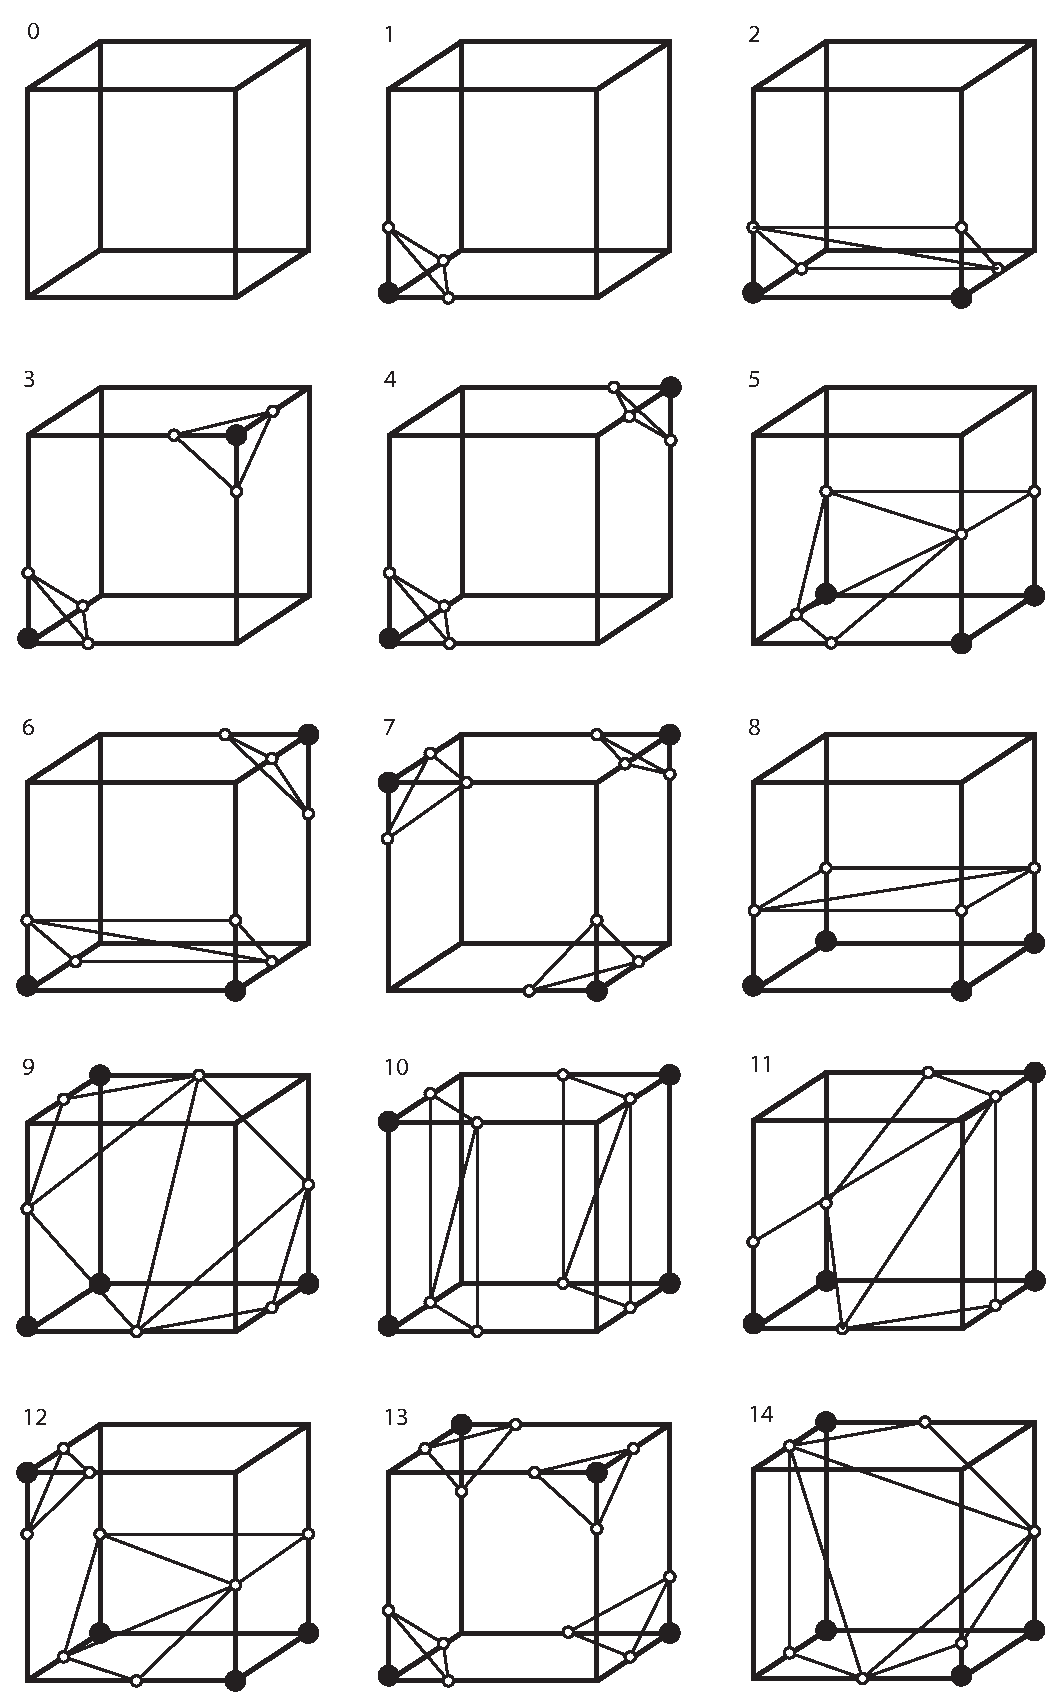
\includegraphics[scale=0.5]{Figures/marching_cubes.eps}
				\caption{Marching cubes}
		\end{center}
			\label{MarchingCubes}
		\end{figure}
		
	\subsection{C\#/.Net and XNA}
	The executable files for this project was written the programming language C\# and Microsoft .NET was utilized as a framework. To make graphics easier to display the environment Microsoft XNA was used. 

\section{System description}

	\subsection{System}
	The system that we have built is a fluid represented by particles. Different forces act on the particles which causes them to move the way they do. Fluids are materials that are being deformed under forces. They are commonly known to be liquids but fluids are also gases. Our model is capable simulating a gas like substance. However, the focus was mainly on creating a liquid. Normally, a simulation system is described with a bond graph or block diagram. In our case though, because this is a particle based fluid simulation, which requires quite a lot of particles to look like liquid, it is hard.

	
	%\subsection{Model}

	\subsection{Physical history}
	One method to describe how fluids behave (describe the motion of substances) is the Navier-Stokes equations, named after Claude-Louis Navier and George Gabriel Stokes. This method is used for this project.

	As seen in the equation below, the physical quantities used are pressure, density and viscosity.
	
	
	\begin{equation}
	\rho\left(\frac{\partial v}{\partial t} + v \cdot\nabla v\right) = -\nabla p + \rho g	 + \mu\nabla^{2}v
\label{eq:}
\end{equation}

This equation is then simplified, as suggested by M�ller03 to:

\begin{equation}
\textbf{a}_{i} = \frac{d\textbf{v}_{i}}{dt} = \frac{-\nabla p_{i} + \rho_{i}\textbf{g}+\mu \nabla^{2}\textbf{v}_{i}}{\rho_{i}}
\label{eq:}
\end{equation}

Where $-\nabla p_{i}$ is force due to pressure, $\rho_{i}\textbf{g}$ is external forces such as gravity and $\mu\nabla^{2}\textbf{v}_{i}$ is force due to visosity.

	\subsection{Density}
The first step in the simulation is computing the particle densities. By substituting $A$ in equation x with the particle density $\rho$, we get:
\begin{equation}
	\rho_{S}(\textbf{r}) = {\sum_{j}} m_{j}W(\textbf{r}-\textbf{r}_{j},h)
\label{eq:}
\end{equation}
The smoothing kernel used for calculating the density in this simulation was the $W_{poly6}$ kernel, designed by M�ller03.

\begin{equation}
	\rho_{S}(\textbf{r}) = {\sum_{j}} m_{j}W(\textbf{r}-\textbf{r}_{j},h)
\label{eq:}
\end{equation}

	\subsection{Pressure}
	The pressure is calculating using the forumla described below. This is a simplified version of the original SPH formula to calculate the pressure. \cite{muller} 
	\begin{equation}
		p = k(\rho - \rho{_0})
	\label{eq:}
	\end{equation}
	
	where $\rho$ is the density of the current particle, $\rho{_0}$ is the rest density, and $k$ is the gas constant of the current substance being simulated, which depends on the temperature. The higher the temperature, the lighter the substance.
	
	\subsection{Viscosity}
	Viscosity is caused by friction which converts the particle's kinetic energy to heat.
	The viscosity is calculated by looking at the force in the gradient of the neighbors of each particle.
	
	\subsection{Force simulation}
	The sum of all forces that act on the particles is used for the final calculation that will actually move a particle. The force is recalculated according to Newtons 2nd law to acceleration. The current acceleration is multiplied with a predefined timestep and added to the current velocity. The new velocity is multipled with the same predefined timestep, which gives the movement ant therefore the new position of the particle.
	
		
\section{Implementation}
	
	As mentioned in methods, code fot this simulation were written in C\# using Microsoft Visual Studion Pro 2010.	

	\subsection{Structure of the simulation software}
	The main functions of the software for this simulation is to calculate the forces which affect the particles. The amount of forces acting on each particle depends on the surrounding particles, and therefore an important step is to find the neighbors of each particle. A particle i is considered as neighbour to a particle j if the distance betweem them is less than a preset maximum distance. The distance between found neighbours decides how they will affect eachother.
	

	\subsection{Collision Handling}
	The collision handling performed in this simulation is fairly simple. A bound is defined in which the fluid can exist. After a particle's new position is calculated, the program checks if it is within the acceptable bounds or not. If the particle's position is not within the defined area, the velocity and acceleration of the particle is inverted, otherwise nothing changes.

	\subsection{Changing simulation behaviour}
 To make the simulation interactive, sliders were added to the simulation software GUI, which changes the values of constants used in the equations calculating the forces of the simulation.

	
	\subsection{Rendering}
	The simulation is rendered using the benefits of XNA. A "camera" is created to capture the visual implementation of the simulation. XNA Studio already provides with shaders which really adds to the visual appearance without being coded manually.


\section{Results}
The result of this project is an executable .NET-application. This means it can be run on any computer as long as that computer has the .NET framework installed, along with XNA Studio. Screenshots from the resulting application of this project is presented the appendix.
\textbf{Figure 2} demonstrates the general appearance of the program. In the middle there are a number of blue particles sealed in a transparent cube. (An orange grid is passing under the cube). In the top left the user will find statistics from the calculation of the program as well as tips on how to control the program. In the top right there are six different sliders and one button.
Figure 3 shows a close-up of the top left of the program. The label FPS stands for frames per second and is a measurement of how many frames per second the CPU manages to calculate. A higher FPS-total will give a more fluent appearance then a low. Performance of the application may vary as different computers have different specifications and as a result get a higher or lower FPS when the particles are in motion. StopWatch. The label named Particles shows the number of particles. Camera Position has the three variables X, Y and Z, measuring the cameras position from the centre of the cube. The user can control the camera using the arrows on the keyboard. The user can also toggle to fullscreen, pressing <F6> as well as toggle grid on and off, pressing <tab>. Pressing <shift> will toggle marching cubes on and off.
Figure 4 shows a close-up of the top right. The user can drag the three first sliders (from the top) to control the fluid parameters. Particles control the number of particles. Time step controls the speed of the simulation. Dragging the Rotation speed slider will rotate the cube clockwise or counter clockwise. There is also a Restart-button that will restart the simulation. Pressing restart will not restore the changes the user have done on any of the sliders or keyboard commands.


\section{Conclusion}
- Producing realistic simulation of fluids is very difficult. It is also hard to define what a "good" simulation is. There are several other simulations, often published as short demonstration films that are pre-rendered and not interactive. An example of that is the result of Beaudoin, Clavet and Poulin (2005). Beaudoin et al produces stunning visuals and the clip has gotten 23 956 views on youtube.com (2011-03-09) which certainly could be rubricated as "good". With that in mind we think that our own result is good. We have succeeded in reaching the aim of our project.

What could have been done differently?
-  One could consider if the same, or better, result could be accomplished if another environment had been chosen as a platform for the project. For example if we have had chosen OpenGL instead of XNA. It was also possible to have used other methods to reach our goal. One of the most important reasons why we chose to use SPH was that there were quite a lot of resources available on the subject. At one point we were considering using point splatting (M�ller at alt, 2003) instead of marching cubes. But we quickly realized that point splatting generally uses 10.000 to 100.000 particles, which would have demanded significantly more CPU-power, since we only used up to 2000 particles in our system.
If we wanted to continue developing the software, what would we have done?
- In an ongoing development of the project we would concentrate our efforts to implement the NVIDIA engine CUDA, Compute Unified Device Architecture, to the project. CUDA uses the inbuilt graphics card of the computer to calculate simple computations and unburden the CPU. Doing this will improve the "speed" of the simulation, i.e. the number of frames/second. We would also do more collision handling. We could for example have a static object in the glass cube that the fluid would have to interact with.

Rewritten!\\

	As a conclusion, producing realistic fluid simulations is difficult. It is also hard to define what is considered a correct simulation. Our refence point as to how a good fluid simulation should look like is the simulation done by Beaudoin, Clavet and Poulin in 2005. %Our expectations were not to create such a simulation
	Moreover, we could have taken other approaches to achieve different results, better or worse. We used XNA as a platform for our project, however there are other options that we could have chosen, OpenGL for instance. 
\newpage

\section{References}

\begin{thebibliography}{20}

\bibitem{muller}
M�ller M., Charypar D., Gross M.
\emph{Particle based fluid simulation for interactive applications}
2003.

\bibitem{lucy}
Lucy L. B.
\emph{A numerical approach to the testing of the fission hypothesis.}
The Astronomical Journal, 82:1013-1024, 1977.
\url{http://adsabs.harvard.edu/full/1977AJ.....82.1013L}

\bibitem{sph}
Gingold R. A., Monaghan J. J.
\emph{Smoothed Particle hydrodynamics: theory and application t non-spherical stars.}
Monthly Notices of the Royal Astronomical Society, 181:375-389, 1977.
\url{http://adsabs.harvard.edu/full/1977MNRAS.181..375G}(2011-03-09)

\bibitem{marching_cubes}
Cline H. E., Lorensen W.E.
\emph{Marching Cubes: A high resolution 3D surface construction algorithm.} 
SIGGRAPH, 1987.
\url{http://kucg.korea.ac.kr/seminar/2001/src/PA-01-16.pdf}(2011-03-09)

\bibitem{visco_fluid_simulation}
Beaudoin P., Clavet S., Poulin P.
\emph{Particle-based Viscoelastic Fluid Simulation.}
\url{http://www.iro.umontreal.ca/labs/infographie/papers/Clavet-2005-PVFS/pvfs.pdf}(2011-01)
\end{thebibliography}

\newpage
\appendix
\section{Screen captures}

\end{document}